\hyperdef{cond}{prob}{\section{Conditional Probability}}

Suppose that we pick a random person in the world.  Everyone has an
equal chance of being selected.  Let $A$ be the event that the person
is an MIT student, and let $B$ be the event that the person lives in
Cambridge.  What are the probabilities of these events?  Intuitively,
we're picking a random point in the big ellipse shown below and asking
how likely that point is to fall into region $A$ or $B$:
%
\begin{center}
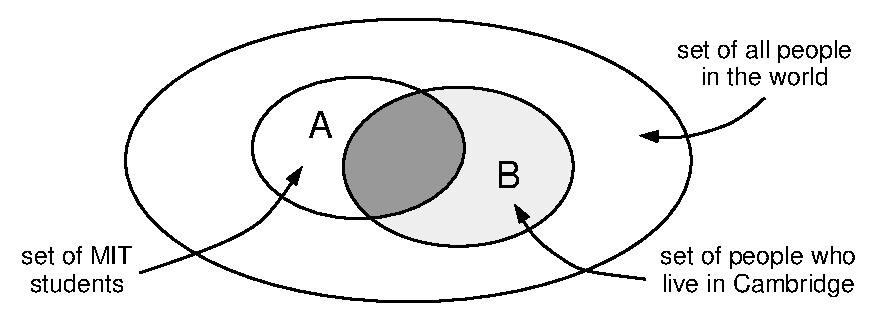
\includegraphics[height=2in]{figures/cambridge-conditional}
\end{center}
%
The vast majority of people in the world neither live in Cambridge nor
are MIT students, so events $A$ and $B$ both have low probability.
But what is the probability that a person is an MIT student,
\textit{given} that the person lives in Cambridge?  This should be
much greater--- but what is it exactly?

What we're asking for is called a \term{conditional probability}; that
is, the probability that one event happens, given that some other
event definitely happens.  Questions about conditional probabilities
come up all the time:
%
\begin{itemize}
\item What is the probability that it will rain this afternoon, given
that it is cloudy this morning?
\item What is the probability that two rolled dice sum to 10, given
that both are odd?
\item What is the probability that I'll get four-of-a-kind in Texas No
Limit Hold 'Em Poker, given that I'm initially dealt two queens?
\end{itemize}

There is a special notation for conditional probabilities.  In
general, $\prcond{A}{B}$ denotes the probability of event $A$, given
that event $B$ happens.  So, in our example, $\prcond{A}{B}$ is the
probability that a random person is an MIT student, given that he or
she is a Cambridge resident.

How do we compute $\prcond{A}{B}$?  Since we are \textit{given} that
the person lives in Cambridge, we can forget about everyone in the
world who does not.  Thus, all outcomes outside event $B$ are
irrelevant.  So, intuitively, $\prcond{A}{B}$ should be the fraction
of Cambridge residents that are also MIT students; that is, the answer
should be the probability that the person is in set $A \intersect B$ (darkly
shaded) divided by the probability that the person is in set $B$
(lightly shaded).  This motivates the definition of conditional
probability:
\begin{definition}\label{LN12:prcond}
\[
\prcond{A}{B} \eqdef \frac{\pr{A \intersect B}}{\pr{B}}
\]
\end{definition}
If $\pr{B} = 0$, then the conditional probability $\prcond{A}{B}$ is
undefined.

Pure probability is often counterintuitive, but conditional probability is
worse!  Conditioning can subtly alter probabilities and produce unexpected
results in randomized algorithms and computer systems as well as in
betting games.  Yet, the mathematical definition of conditional
probability given above is very simple and should give you no trouble---
provided you rely on formal reasoning and not intuition.

\subsection{The Halting Problem}

The {\em Halting Problem} is the canonical undecidable problem in
computation theory that was first introduced by Alan Turing in his seminal
1936 paper.  The problem is to determine whether a Turing machine halts on
a given \dots blah, blah, blah.  But what's \textit{much more important},
it is the name of the MIT EECS department's famed C-league hockey team.

In a best-of-three tournament, the Halting Problem wins the first game
with probability $1/2$.  In subsequent games, their
probability of winning is determined by the outcome of the previous
game.  If the Halting Problem won the previous game, then they are
invigorated by victory and win the current game with probability
$2/3$.  If they lost the previous game, then they are
demoralized by defeat and win the current game with probablity only
$1/3$.  What is the probability that the Halting Problem wins
the tournament, given that they win the first game?


This is a question about a conditional probability.  Let $A$ be the
event that the Halting Problem wins the tournament, and let $B$ be the
event that they win the first game.  Our goal is then to determine the
conditional probability $\prcond{A}{B}$.

We can tackle conditional probability questions just like ordinary
probability problems: using a tree diagram and the four step method.
A complete tree diagram is shown below, followed by an explanation of
its construction and use.
%
\begin{center}
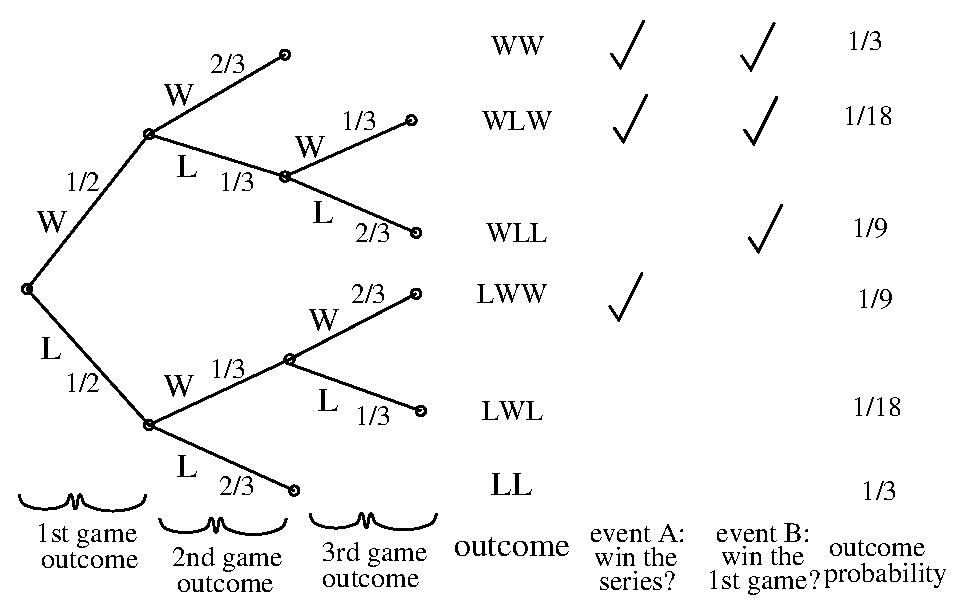
\includegraphics[height=3in]{figures/hockey} % redo this
\end{center}

\subsubsection*{Step 1:  Find the Sample Space}

Each internal vertex in the tree diagram has two children, one
corresponding to a win for the Halting Problem (labeled $W$) and one
corresponding to a loss (labeled $L$).  The complete sample space is:
%
\[
\sspace = \set{ WW,\ WLW,\ WLL,\ LWW,\ LWL,\ LL }
\]

\subsubsection*{Step 2:  Define Events of Interest}

The event that the Halting Problem wins the whole tournament is:
%
\[
T = \set{WW,\ WLW,\ LWW} \\
\]
%
And the event that the Halting Problem wins the first game is:
%
\[
F = \set{WW, WLW, WLL }
\]
%
The outcomes in these events are indicated with checkmarks in the tree
diagram.

\subsubsection*{Step 3:  Determine Outcome Probabilities}

Next, we must assign a probability to each outcome.  We begin by
labeling edges as specified in the problem statement.  Specifically,
The Halting Problem has a $1/2$ chance of winning the first game, so
the two edges leaving the root are each assigned probability $1/2$.
Other edges are labeled $1/3$ or $2/3$ based on the outcome of the
preceding game.  We then find the probability of each outcome by
multiplying all probabilities along the corresponding root-to-leaf
path.  For example, the probability of outcome $WLL$ is:
%
\[
\frac{1}{2} \cdot \frac{1}{3} \cdot \frac{2}{3} = \frac{1}{9}
\]

\subsubsection*{Step 4: Compute Event Probabilities}

We can now compute the probability that The Halting Problem wins the
tournament, given that they win the first game:
%
\begin{align*}
\prcond{A}{B}
    & = \frac{\pr{A \intersect B}}{\pr{B}} \\
    & = \frac{\pr{\set{WW, WLW}}}{\pr{\set{WW, WLW, WLL}}} \\
    & = \frac{1/3 + 1/18}{1/3 + 1/18 + 1/9} \\
    & = \frac{7}{9}
\end{align*}
%
We're done!  If the Halting Problem wins the first game, then they win
the whole tournament with probability $7 / 9$.  


\subsection{Why Tree Diagrams Work}

We've now settled into a routine of solving probability problems using
tree diagrams.  But we've left a big question unaddressed: what is the
mathematical justification behind those funny little pictures?  Why do
they work?

The answer involves conditional probabilities.  In fact, the
probabilities that we've been recording on the edges of tree diagrams
\textit{are} conditional probabilities.  For example, consider the
uppermost path in the tree diagram for the Halting Problem, which
corresponds to the outcome $WW$.  The first edge is labeled $1/2$,
which is the probability that the Halting Problem wins the first game.
The second edge is labeled $2 / 3$, which is the probability that the
Halting Problem wins the second game, \textit{given} that they won the
first--- that's a conditional probability!  More generally, on each
edge of a tree diagram, we record the probability that the experiment
proceeds along that path, given that it reaches the parent vertex.

So we've been using conditional probabilities all along.  But why can
we multiply edge probabilities to get outcome probabilities?  For
example, we concluded that:
%
\begin{align*}
\pr{WW} & = \frac{1}{2} \cdot \frac{2}{3} \\
	& = \frac{1}{3}
\end{align*}
%
Why is this correct?

The answer goes back to Definition~\ref{LN12:prcond} of conditional probability
which could be written in a form called the \term{Product Rule} for
probabilities:
%
\begin{rul*}[Product Rule for 2 Events]
If $\pr{E_1} \neq 0$, then:
%
\[
\pr{E_1 \intersect E_2} = \pr{E_1} \cdot \prcond{E_2}{E_1}
\]
\end{rul*}
%
Multiplying edge probabilities in a tree diagram amounts to evaluating
the right side of this equation.  For example:
%
\begin{align*}
\lefteqn{\pr{\text{win first game} \intersect \text{win second game}}}
		\hspace{0.5in} \\
	& = \pr{\text{win first game}} \cdot
            \prcond{\text{win second game}}{\text{win first game}} \\
	& = \frac{1}{2} \cdot \frac{2}{3}
\end{align*}
%
So the Product Rule is the formal justification for multiplying edge
probabilities to get outcome probabilities!  Of course to justify
multiplying edge probabilities along longer paths, we need a Product Rule
for $n$ events.  The pattern of the $n$ event rule should be apparent from
\begin{rul*}[Product Rule for 3 Events]
\[
\pr{E_1 \intersect E_2 \intersect E_3}
   = \pr{E_1} \cdot \prcond{E_2}{E_1} \cdot \prcond{E_3}{E_2 \intersect E_1}
\]
providing $\pr{E_1 \intersect E_2} \neq 0$.
\end{rul*}
This rule follows from the definition of conditional probability and the
trivial identity
\[
\pr{E_1 \intersect E_2 \intersect E_3} =
\pr{E_1}\cdot \frac{\pr{E_2 \intersect E_1}}{\pr{E_1}} \cdot
      \frac{\pr{E_3 \intersect E_2 \intersect E_1}}{\pr{E_2 \intersect E_1}}
\]


\subsection{The Law of Total Probability}

Breaking a probability calculation into cases simplifies many problems.
The idea is to calculate the probability of an event $A$ by splitting into
two cases based on whether or not another event $E$ occurs.  That is,
calculate the probability of $A \intersect E$ and $A \intersect \bar{E}$.
By the Sum Rule, the sum of these probabilities equals $\pr{A}$.
Expressing the intersection probabilities as conditional probabilities yields
\begin{rul*}[Total Probability]
\[
\pr{A} = \prcond{A}{E} \cdot \pr{E} +
         \prcond{A}{\bar{E}} \cdot \pr{\bar{E}}.
\]
\end{rul*}

For example, suppose we conduct the following experiment.  First, we flip a
coin.  If heads comes up, then we roll one die and take the result.  If
tails comes up, then we roll two dice and take the sum of the two results.
What is the probability that this process yields a 2?  Let $E$ be the
event that the coin comes up heads, and let $A$ be the event that we get a
2 overall.  Assuming that the coin is fair, $\pr{E} = \pr{\bar{E}} = 1/2$.
There are now two cases. If we flip heads, then we roll a 2 on a single
die with probabilty $\prcond{A}{E} = 1/6$.  On the other hand, if we flip
tails, then we get a sum of 2 on two dice with probability
$\prcond{A}{\bar{E}} = 1/36$.  Therefore, the probability that the whole
process yields a 2 is
\[
\pr{A} = \frac{1}{2} \cdot \frac{1}{6} + \frac{1}{2} \cdot \frac{1}{36} =
  \frac{7}{72}.
\]

There is also a form of the rule to handle more than two cases.
\begin{rul*}[Multicase Total Probability]
If $E_1, \dots, E_n$ are pairwise disjoint events whose
union is the whole sample space, then:
\[
\pr{A} = \sum_{i=1}^{n} \prcond{A}{E_i} \cdot \pr{E_i}.
\]

\end{rul*}

\iffalse

\subsection{\textit{A Posteriori} Probabilities}

Suppose that we turn the hockey question around: what is the
probability that the Halting Problem won their first game, given that
they won the series?

This seems like an absurd question!  After all, if the Halting Problem
won the series, then the winner of the first game has already been
determined.  Therefore, who won the first game is a question of fact,
not a question of probability.  However, our mathematical theory of
probability contains no notion of one event preceding another--- there
is no notion of time at all.  Therefore, from a mathematical
perspective, this is a perfectly valid question.  And this is also a
meaningful question from a practical perspective.  Suppose that you're
told that the Halting Problem won the series, but not told the results
of individual games.  Then, from your perspective, it makes perfect
sense to wonder how likely it is that The Halting Problem won the
first game.

A conditional probability $\prcond{B}{A}$ is called  \term{a
posteriori} if event $B$ precedes event $A$ in time.  Here are some
other examples of a posteriori probabilities:
%
\begin{itemize}
\item The probability it was cloudy this morning, given that it rained
in the afternoon.
\item The probability that I was initially dealt two queens in Texas
No Limit Hold 'Em poker, given that I eventually got four-of-a-kind.
\end{itemize}
%
Mathematically, a posteriori probabilities are \textit{no different}
from ordinary probabilities; the distinction is only at a higher,
philosophical level.  Our only reason for drawing attention to them is
to say, ``Don't let them rattle you.''

Let's return to the original problem.  The probability that the
Halting Problem won their first game, given that they won the series
is $\prcond{B}{A}$.  We can compute this using the definition of
conditional probability and our earlier tree diagram:
%
\begin{align*}
\prcond{B}{A} & = \frac{\pr{B \intersect A}}{\pr{A}} \\
              & = \frac{1/3 + 1/18}{1/3 + 1/18 + 1/9} \\
              & = \frac{7}{9}
\end{align*}

This answer is suspicious!  In the preceding section, we showed that
$\prcond{A}{B}$ was also $7/9$.  Could it be true that $\prcond{A}{B}
= \prcond{B}{A}$ in general?  Some reflection suggests this is
unlikely.  For example, the probability that I feel uneasy, given that
I was abducted by aliens, is pretty large.  But the probability that I
was abducted by aliens, given that I feel uneasy, is rather small.

Let's work out the general conditions under which $\prcond{A}{B} =
\prcond{B}{A}$.  By the definition of conditional probability, this
equation holds if an only if:
%
\[
\frac{\pr{A \intersect B}}{\pr{B}} = \frac{\pr{A \intersect B}}{\pr{A}}
\]
%
This equation, in turn, holds only if the denominators are equal or
the numerator is 0:
%
\[
\pr{B} = \pr{A}
\hspace{0.25in} \text{or} \hspace{0.25in}
\pr{A \intersect B} = 0
\]
%
The former condition holds in the hockey example; the probability that
the Halting Problem wins the series (event $A$) is equal to the
probability that it wins the first game (event $B$).  In fact, both
probabilities are $1/2$.

\iffalse
Such pairs of probabilities are related by Bayes' Rule:
%
\begin{theorem}[Bayes' Rule]
If $\pr{A}$ and $\pr{B}$ are nonzero, then:
%
\[
\prcond{A}{B} \cdot \pr{B} = \prcond{B}{A} \cdot \pr{A}
\]
\end{theorem}

\begin{proof}
When $\pr{A}$ and $\pr{B}$ are nonzero, both sides are equal to $\pr{A
\intersect B}$ and thus are equal to each other.
\end{proof}

In the hockey problem, the probability that the Halting Problem wins the
first game is $1/2$ and so is the probability that the Halting Problem
wins the series.  Therefore, $\pr{A} = \pr{B} = 1/2$.  This, together with
Bayes' Rule, explains why $\pr{A mid B}$ and $\prcond{B}{A}$ turned out to
be equal in the hockey example.  \fi
\fi

\iffalse

\subsection{A Coin Problem}
Someone hands you either a fair coin or a 
trick coin with heads on both sides.  You flip
the coin 100 times and see heads every time.  What can you say about
the probability that you flipped the fair coin?  Remarkably---
nothing!

In order to make sense out of this outrageous claim, let's formalize
the problem.  The sample space is worked out in the tree diagram
below.  We do not know the probability that you were handed the fair
coin initially--- you were just given one coin or the other--- so
let's call that $p$.
%
\begin{center}
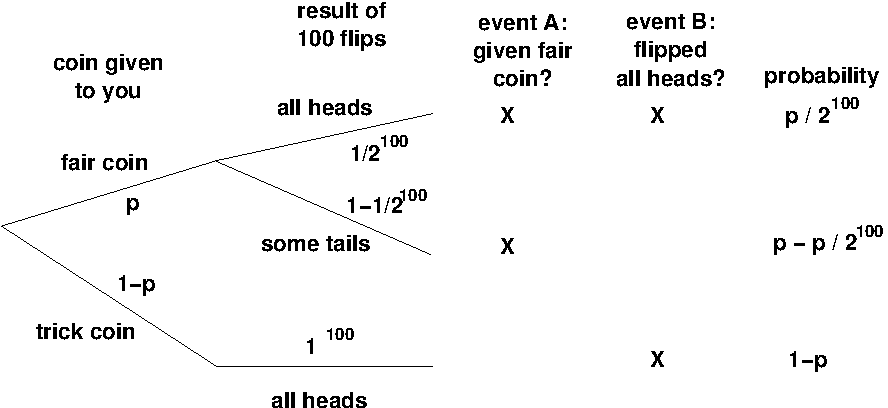
\includegraphics{figures/trick-coin}
\end{center}
%
Let $A$ be the event that you were handed the fair coin, and let $B$
be the event that you flipped 100 heads.  Now, we're looking for
$\prcond{A}{B}$, the probability that you were handed the fair coin,
given that you flipped 100 heads.  The outcome probabilities are
worked out in the tree diagram.  Plugging the results into the
definition of conditional probability gives:
%
\begin{align*}
\prcond{A}{B}	& = \frac{\pr{A \intersect B}}{\pr{B}} \\
		& = \frac{p / 2^{100}}{1 - p + p / 2^{100}} \\
		& = \frac{p}{2^{100} (1 - p) + p}
\end{align*}
%
This expression is very small for moderate values of $p$ because of
the $2^{100}$ term in the denominator.  For example, if $p = 1/2$,
then the probability that you were given the fair coin is essentially
zero.

But we \textit{do not know} the probability $p$ that you were given
the fair coin.  And perhaps the value of $p$ is \textit{not} moderate;
in fact, maybe $p = 1 - 2^{-100}$.  Then there is nearly an even
chance that you have the fair coin, given that you flipped 100 heads.
In fact, maybe you were handed the fair coin with probability $p = 1$.
Then the probability that you were given the fair coin is, well, 1!

A similar problem arises in polling before an election.  A pollster
picks a random American and asks his or her party affiliation.  If
this process is repeated many times, what can be said about the
population as a whole?  To clarify the analogy, suppose that the
country contains only two people.  There is either one Republican and
one Democrat (like the fair coin), or there are two Republicans (like
the trick coin).  The pollster picks a random citizen 100 times, which
is analogous to flipping the coin 100 times.  Suppose that he picks a
Republican every single time.  However, even given this
polling data, the probability that there is one citizen in each party
could still be anywhere between 0 and 1!

What the pollster \textit{can} say is that either:
%
\begin{enumerate}
\item Something earth-shatteringly unlikely happened during the poll.
\item There are two Republicans.
\end{enumerate}
%
This is as far as probability theory can take us; from here, you must
draw your own conclusions.  Based on life experience, many people
would consider the second possibility more plausible.  However, if you
are just \textit{convinced} that the country isn't entirely Republican
(say, because you're a citizen and a Democrat), then you might believe
that the first possibility is actually more likely.
\fi


\subsection{Medical Testing}

There is an unpleasant condition called \emph{BO} suffered by 10\% of the
population.  There are no prior symptoms; victims just suddenly start to
stink.  Fortunately, there is a test for latent \emph{BO} before things
start to smell.  The test is not perfect, however:
\begin{itemize}

\item If you have the condition, there is a 10\% chance
that the test will say you do not.  (These are called ``false
negatives''.)

\item If you do not have the condition, there is a 30\% chance that the test
will say you do.  (These are ``false positives''.)

\end{itemize}

Suppose a random person is tested for latent \emph{BO}.  If the test is
positive, then what is the probability that the person has the condition?

\subsubsection*{Step 1: Find the Sample Space}

The sample space is found with the tree diagram below.
%
\begin{center}
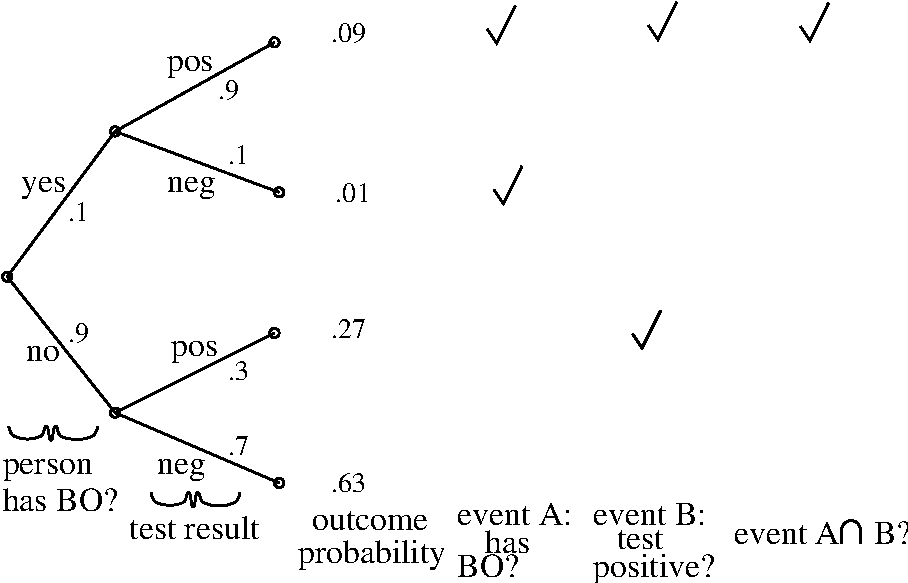
\includegraphics[height=3in]{figures/BO}
\end{center}

\subsubsection*{Step 2: Define Events of Interest}

Let $A$ be the event that the person has \emph{BO}.  Let $B$ be the
event that the test was positive.  The outcomes in each event are marked
in the tree diagram.  We want to find $\prcond{A}{B}$, the probability
that a person has \emph{BO}, given that the test was positive.

\subsubsection*{Step 3: Find Outcome Probabilities}

First, we assign probabilities to edges.  These probabilities are drawn
directly from the problem statement.  By the Product Rule, the
probability of an outcome is the product of the probabilities on the
corresponding root-to-leaf path.  All probabilities are shown in the
figure.

\subsubsection*{Step 4: Compute Event Probabilities}
p
\begin{align*}
\prcond{A}{B}	& = \frac{\pr{A \intersect B}}{\pr{B}} \\
		& = \frac{0.09}{0.09 + 0.27} \\
		& = \frac{1}{4}
\end{align*}
%
If you test positive, then there is only a 25\% chance that you have
the condition!

This answer is initially surprising, but makes sense on reflection.
There are two ways you could test positive.  First, it could be that
you are sick and the test is correct.  Second, it could be that you
are healthy and the test is incorrect.  The problem is that almost
everyone is healthy; therefore, most of the positive results arise
from incorrect tests of healthy people!

We can also compute the probability that the test is correct for a
random person.  This event consists of two outcomes.  The person could
be sick and the test positive (probability $0.09$), or the person
could be healthy and the test negative (probability $0.63$).
Therefore, the test is correct with probability $0.09 + 0.63 = 0.72$.
This is a relief; the test is correct almost three-quarters of the
time.

But wait!  There is a simple way to make the test correct 90\% of the
time: always return a negative result!  This ``test'' gives the right
answer for all healthy people and the wrong answer only for the 10\%
that actually have the condition.  The best strategy is to completely
ignore the test result!

There is a similar paradox in weather forecasting.  During winter,
almost all days in Boston are wet and overcast.  Predicting miserable
weather every day may be more accurate than really trying to get it
right!

\subsection{Conditional Identities}

The probability rules above extend to probabilities conditioned on the
same event.  For example, the Inclusion-Exclusion formula for two sets
holds when all probabilities are conditioned on an event $C$:
\[
\prcond{A \cup B}{C} = \prcond{A}{C} + \prcond{B}{C} - \prcond{A \intersect B}{C}.
\]
This follows from the fact that if $\pr{C} \neq 0$ and we define
\[
\prsub{A}{C} \eqdef \prcond{A}{C}
\]
then $\prsub{}{C}$ satisfies the definition of being probability function.

\iffalse
It is important not to mix up events before and after the conditioning bar.
For example, the following is \textit{not} a valid identity:
%
\begin{falseclm*}
\begin{equation}\label{LN12:fc}
\prcond{A}{B \cup C} = \prcond{A}{B} + \prcond{A}{C} - \prcond{A}{B \intersect C}.
\end{equation}
\end{falseclm*}

\begin{notesproblem}
Give a simple counterexample to~\eqref{LN12:fc}.
\end{notesproblem}
\fi
%

\iffalse
A counterexample is shown below.  In this case, $\prcond{A}{B} = 1$,
$\prcond{A}{C} = 1$, and $\prcond{A}{B \cup C} = 1$.  However, since
$1 \neq 1 + 1$, the equation above does not hold.
%
\begin{center}
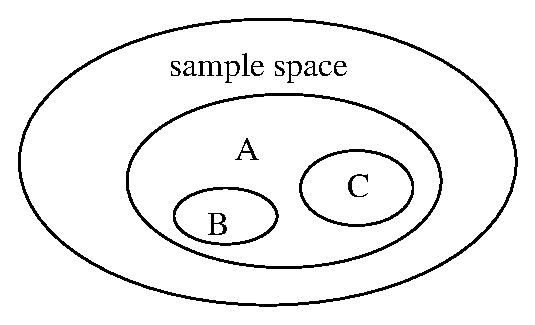
\includegraphics[height=1.5in]{figures/cx19}
\end{center}
%
So you're convinced that this equation is false in general, right?
Let's see if you \textit{really} believe that.

\subsection{Discrimination Lawsuit}

Several years ago there was a sex discrimination lawsuit against
Berkeley.  A female professor was denied tenure, allegedly because she
was a woman.  She argued that in every one of Berkeley's 22
departments, the percentage of male applicants accepted was greater
than the percentage of female applicants accepted.  This sounds very
suspicious!

However, Berkeley's lawyers argued that across the whole university
the percentage of male tenure applicants accepted was actually
\textit{lower} than the percentage of female applicants accepted.
This suggests that if there was any sex discrimination, then it was
against men!  Surely, at least one party in the dispute must be lying.

Let's simplify the problem and express both arguments in terms of
conditional probabilities.  Suppose that there are only two
departments, EE and CS, and consider the experiment where we pick a
random applicant.  Define the following events:
%
\begin{itemize}
\item Let $A$ be the event that the applicant is accepted.
\item Let $F_{EE}$ the event that the applicant is a female applying to EE.
\item Let $F_{CS}$ the event that the applicant is a female applying to CS.
\item Let $M_{EE}$ the event that the applicant is a male applying to EE.
\item Let $M_{CS}$ the event that the applicant is a male applying to
CS.
\end{itemize}
%
Assume that all applicants are either male or female, and that no
applicant applied to both departments.  That is, the events $F_{EE}$,
$F_{CS}$, $M_{EE}$, and $M_{CS}$ are all disjoint.

In these terms, the plaintiff is make the following argument:
%
\begin{align*}
\prcond{A}{F_{EE}} & < \prcond{A}{M_{EE}} \\
\prcond{A}{F_{CS}} & < \prcond{A}{M_{CS}}
\end{align*}
%
That is, in both departments, the probability that a woman is accepted
for tenure is less than the probability that a man is accepted.  The
university retorts that overall a woman applicant is \textit{more}
likely to be accepted than a man:
%
\[
\prcond{A}{F_{EE} \cup F_{CS}} > \prcond{A}{M_{EE} \cup M_{CS}}
\]

It is easy to believe that these two positions are contradictory.  In
fact, we might even try to prove this by adding the plaintiff's two
inequalities and then arguing as follows:
%
\begin{align*}
&& \prcond{A}{F_{EE}} + \prcond{A}{F_{CS}} & < 
	\prcond{A}{M_{EE}} + \prcond{A}{M_{CS}} \\
\Rightarrow && 
\prcond{A}{F_{EE} \cup F_{CS}} & <
	\prcond{A}{M_{EE} \cup M_{CS}}
\end{align*}
%
The second line exactly contradicts the university's position!  But there
is a big problem with this argument; the second inequality follows from
the first only if we accept the false identity~\eqref{LN12:fc}.  This argument
is bogus!  Maybe the two parties do not hold contradictory positions after
all!

In fact, the table below shows a set of application statistics for
which the assertions of both the plaintiff and the university hold:
%
\[
\begin{array}{crr}
\mbox{CS} & \mbox{0 females accepted, 1 applied} & 0\% \\
          & \mbox{50 males accepted, 100 applied} & 50\% \\
\mbox{EE} & \mbox{70 females accepted, 100 applied} & 70\% \\
          & \mbox{1 male accepted, 1 applied} & 100\% \\
\hline
\mbox{Overall} & \mbox{70 females accepted, 101 applied} & \approx 70\% \\
          & \mbox{51 males accepted, 101 applied} & \approx 51\%
\end{array}
\]
%
In this case, a higher percentage of males were accepted in both
departments, but overall a higher percentage of females were accepted!
Bizarre!
\fi

\endinput